\documentclass[conference]{./sty/IEEEtran}
% \documentclass[a4]{article}
\renewcommand{\baselinestretch}{1.15}

% pour les accents utilisés en français
\usepackage[utf8]{inputenc}
\usepackage[T1]{fontenc}

% pour inclure joliment un algorithme
\usepackage{url}
\usepackage[a4paper,pagebackref,bookmarksnumbered]{hyperref} % ps2pdf
% pour inclure joliment un algorithme
\usepackage{algorithmic}
\usepackage[pdftex]{graphicx}
\usepackage{cite}

\usepackage{array}
\usepackage{booktabs}

% Si Latex ne fait pas correctement la césure de certains mots,
% indiquez les emplacements corrects pour les tirets dans ces mots
\hyphenation{op-tical net-works semi-conduc-tor}


\begin{document}

\title{Personnalisation de méthodes pédagogiques en e-learning}


\author{
\IEEEauthorblockN{Jérémy Edert, Mathis Paul, Pierre Turpin}
\IEEEauthorblockA{INSA de Lyon}
  % Jérémy Edert, \\
  % Mathis Paul, \\
  % Pierre Turpin
}

\maketitle
\newpage

\tableofcontents
\newpage

\section{Introduction}

Le e-learning se développe de façon importante dans un grand nombre de
domaines, notamment en entreprise pour la formation continue des personnels.
Dans le cadre du projet de synthèse bibliographique, nous cherchons à étudier
et comparer les différentes solutions existantes dans le domaine des systèmes
de recommandation appliqués au e-learning. \\

L'ensemble des fiches de lecture ci-jointes en annexe nous a permis d'établir
cette synthèse et résument les papiers de recherche lus. Ces articles ont été
repris de différentes conférences et journaux et se concentrent sur les trois
thèmes principaux que nous aborderons : la recherche de contenu, l'utilisation
du contexte et des informations de l'utilisateur lors du ciblage, puis
l'application dans le domaine du e-learning. \\

La plupart des articles lus et résumés sont tirés des références de
\cite{DBLP:journals/tlt/VerbertMOWDBD12}. En effet ce dernier regroupe déjà
beaucoup de résultats et de méthodes de recherche contextuelle de documents
pédagogiques pour du e-learning. \\

% TODO bullshiter un peu plus


\section{Utilisation du contexte et des informations de l'utilisateur lors du ciblage}

Pour personnaliser et fiabiliser les résultats de recherche pour un
utilisateur, le contexte et les données utilisateur sont acquis et modifient le
rang des éléments. \\

Le besoin de modéliser proprement et strictement ce genre d'information est
donc devenu nécessaire. Beaucoup de chercheurs étudient et publient des papiers
sur la notion de contexte et sur sa définition la plus exacte possible
\cite{DBLP:journals/tlt/VerbertMOWDBD12},
\cite{DBLP:reference/rsh/AdomaviciusT11},
\cite{DBLP:journals/aim/AdomaviciusMRT11}. \\

\subsection{Connaissance et acquisition du contexte}

Chaque attribut formant le contexte doit avoir sa méthode d'acquisition, de
mise à jour (s'il y en a une) et sa "valeur par défaut" lors de données
manquantes. En effet, toutes ces caractéristiques peuvent être statiques ou
dynamiques, et observables ou peu voire non observables
\cite{DBLP:journals/aim/AdomaviciusMRT11}. Le tableau
\ref{tab:update_observability_context} reprend les caractéristiques possibles
pour un attribut de contexte. \\

\begin{table}
  \centering
  \caption{\label{tab:update_observability_context} Information sur le contexte \cite{DBLP:journals/aim/AdomaviciusMRT11}}
  \begin{tabular}{|p{0.20\linewidth}|p{0.20\linewidth}|p{0.20\linewidth}|p{0.20\linewidth}|}
    \hline
    ~ & Totalement observable & Partiellement observable & Non observable \\ \hline
    Statique & Connaissance totale & Connaissance partielle et statique & Connaissance latente \\ \hline
    Dynamique & Connaissance totale dynamique & Connaissance partielle et dynamique & Aucune connaissance \\ \hline
  \end{tabular}
\end{table}

Les attributs statiques sont des simplifications que le système peut se
permettre car la donnée est considérée comme figée dans le temps le long de
l'utilisation de l'application par un utilisateur. Par exemple une date de
naissance, une identité sont des données fixes pour un utilisateur. Lorsque ces
attributs sont pleinement observables, le système peut considérer les connaître
entièrement. Ce sont les meilleurs cas possibles. S'ils sont partiellement
observables ou peu ou non observables, alors cela implique un retard dans
l'obtention des données plus ou moins grand en fonction de l'observabilité des
attributs. Cependant une fois totalement observés, le système connaît ces
attributs. \\

Les attributs dynamiques sont des données mesurées ayant une certaine durée de
vie. Cette durée dépend de la nature de l'attribut. La localisation
géographique de l'utilisateur n'a pas besoin d'être précise au mètre près. Ce
type d'attribut n'est donc pas à mesurer très fréquemment et comporte une durée
de vie plutôt importante. Mais l'horloge tout simplement est une donnée à
mesurer chaque seconde par définition. Ces différentes mesures deviennent
possible et une large gamme de type d'attribut peut être obtenue par les
nouvelles technologies incluses dans les téléphones et appareils portables
\cite{DBLP:conf/wstst/Kurti08}. \\

Lorsque les attributs ont des valeurs dynamiques, l'observabilité totale permet
d'avoir une connaissance de toute la dynamique de la dimension et donc
d'utiliser avec beaucoup plus de précision cette information. On peut dire que
l'observabilité est totale si le temps d'acquisition de la mesure est plus
petit que sa durée de vie. Cette granularité est à définir par le designer de
l'application en fonction de l'usage fait. Un temps d'acquisition plus lent
entraînera alors une observabilité seulement partielle. La dynamique de l'information
ne pourra être totalement connue et le système devra s'adapter avec des données
manquantes ou anciennes. Pour certains types, les valeurs manquantes peuvent
être inférées et connues \cite{DBLP:journals/prl/TruccoFR99}. Il est à noter
qu'il y a différents niveaux d'observabilité partielle. Ces différences ne sont
pas examiner dans cette synthèse. Lorsque la mesure est non observable, aucune
connaissance ne peut être obtenue et le système doit pouvoir fonctionner avec ce
manque. \\

Il existe deux types de dynamique pour les attributs : dynamique passive et
explicite. \\
Un attribut passivement dynamique peut changer sans agissement
direct de l'utilisateur. En effet, dans le cas d'une géolocalisation,
l'utilisateur n'a pas besoin d'agir directement sur les appareils mobiles pour
changer sa position. Cette valeur est mesurée automatiquement par des capteurs
de positionnement, comme le Global Positionning System (GPS) ou le Wi-Fi
\cite{DBLP:journals/tlt/VerbertMOWDBD12}. \\
Les attributs dont la valeur change via l'action directe de l'utilisateur sont
considérés comme dynamique explicite. C'est le cas en général pour toutes les
informations utilisateurs. Cela peut également correspondre à d'autres types de
données comme des filtres et des préférences que l'utilisateur décrit sur
l'application. Ces données sont, de plus, totalement observables et permettent,
dans le cas des filtres et préférences, d'affiner encore plus les résultats de
recherche proposés. Cela accroit donc l'efficacité de l'application quant au
ciblage. \\

\subsection{Les différents types de contexte}

La notion de contexte a été étudiée dans différentes sciences (psychologie,
intelligence artificielle, modélisation cognitive, ...) et chacune de ces
sciences exprime un point de vue différent
\cite{DBLP:reference/rsh/AdomaviciusT11}. C'est pourquoi nous ne pouvons pas
donner une liste exhaustive des éléments pouvant définir cette notion. Nous
nous baserons principalement sur un nombre fini d'aspects et d'attributs les
plus utilisés dans le cadre des applications de recommandation avec contexte
pour le e-learning. \\

La figure \ref{fig:context} reprend les différents éléments de contexte décrits dans cette section. \\

\begin{figure}[tb]
  \centering
  \caption{\label{fig:context} Modélisation des attributs de contexte \cite{DBLP:journals/tlt/VerbertMOWDBD12}}
  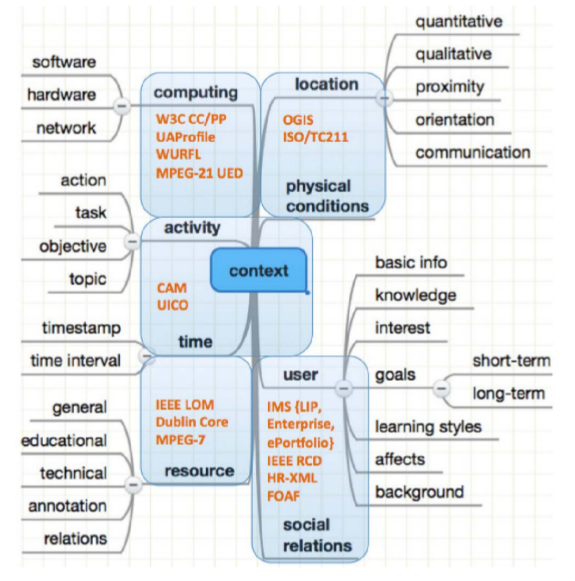
\includegraphics[width=0.5\textwidth]{context}
\end{figure}

\subsubsection{Ordinateur et appareils mobiles}
~\\
Connaître les outils que possède l'utilisateur et utile pour le système de
recommandation. En effet, celui-ci peut ainsi savoir ce qu'il peut recommander.
Cela concerne les capacités réseau, matérielles et logicielles. \\

Au niveau réseau, l'application peut proposer du contenu externe comme des
documents, des vidéos, des supports de présentation ou tout simplement des
pages web. \\

La capacité matérielle -et surtout la différence entre ordinateur et appareil
mobile- est une connaissance importante. Un ordinateur est un outil plus
puissant avec plus de mémoire. L'application peut proposer à l'utilisateur
d'utiliser des logiciels tournant sur ordinateur, ou peut présenter des pages
web lourdes (visualisation 3D par exemple) et peut aussi suggérer un
téléchargement de contenu. \\
Un appareil mobile, même s'il est moins puissant et a moins d'espace de
stockage, possède en revanche une quantité croissante de capteurs utilisables
pour compléter les résultats de recommandation \cite{DBLP:conf/wstst/Kurti08}.
La présentation de l'application ne sera pas non plus faite de la même manière
sur un ordinateur et sur un appareil mobile à cause de la taille de l'écran. \\

Enfin la connaissance des capacités logicielles permet de raffiner les résultats
en soumettant uniquement des recommandations utilisables pour l'utilisateur.
Par exemple des fichiers \emph{Microsoft Office} ne peuvent pas être ouverts sur
toutes les plateformes. \\

\subsubsection{Géolocalisation}
~\\
La position de l'utilisateur à un instant donné est également un élément de contexte important. Il ne s'agit pas forcément de connaitre sa position précise, mais l'environnement dans lequel l'utilisateur se trouve, par exemple se trouve-t-il chez lui, en salle de cours, ou dans la rue ? Se trouve-t-il proche de points d'intérêt qu'il serait intéressant de visiter ? En fonction de l'approche prise par l'application de e-learning, tous ces éléments peuvent avoir leur importance sur le contenu à recommander.\\
Avec l'augmentation des plate-formes mobiles, l'environnement dans lequel se trouve l'utilisateur est devenu une donnée importante du contexte, dont l'acquisition est facilitée par des outils tels que le GPS, ou l'accès Wi-Fi.\cite{DBLP:journals/tlt/VerbertMOWDBD12}\\

\subsubsection{Temps}
~\\
Le contexte temporel consiste en l'heure et la date au moment de l'utilisation. Il peut parfois s'agir d'informations moins précises que ça, telles que la semaine ou le mois \cite{DBLP:journals/tlt/VerbertMOWDBD12}. Par exemple, le matériel proposé à l'utilisateur ne sera pas le même si l'utilisation se fait en pleine journée ou au beau milieu de la nuit. On peut également utiliser cette information en conjonction avec d'autres éléments du contexte. Pour reprendre l'exemple de la géolocalisation, il ne sert à rien de proposer à l'utilisateur de visiter un point d'intérêt si celui-ci est fermé à ce moment-là.\\

\subsubsection{Activité}
~\\
Le contexte d'activité comprend les tâches, objectifs et actions de l'utilisateur. Ces informations permettent tout simplement de mieux filtrer les ressources à recommander afin qu'il puisse atteindre ses objectifs. Quelques modélisations de ce type de contexte ont été proposées, capturant les informations telles que les actions de l'utilisateur aisni que des éléments temporels pour en déduire ss objectifs ou tâches actuels \cite{DBLP:journals/tlt/VerbertMOWDBD12}.\\


\subsubsection{Utilisateur}
~\\
La modélisation du profil de l'élève est un élément fondamental des systèmes
d'e-learning avec personnalisation. L'étude
\cite{DBLP:journals/tlt/VerbertMOWDBD12} s'attache à décrire de façon extensive
les différentes catégories d'informations qu'il est intéressant de prendre en
compte dans ce genre de programme.Outre les informations basiques comme le nom,
l'e-mail, les langues pratiquées ou l'âge, les connaissances de utilisateur sont
un point important à considérer. Il est par ailleurs possible de modéliser
celles-ci avec plus ou moins de précision, par exemple en définissant pour
chaque utilisateur un niveau de compétence pour chaque compétence identifiée
par l'application\cite{DBLP:journals/jucs/SternKHKL10}. \\

Un profil utilisateur peut également comporter des informations relatives à ses
intérêts, ses objectifs d'apprentissage, notamment si la plate-forme
d'e-learning concerne un cursus scolaire comme dans le cas d'une université où
ceux-ci sont clairement définis. La méthode d'apprentissage de l'utilisateur
est aussi une information importante et peut permettre de proposer un contenu
de formation adapté aux différents styles d'apprentissage
\cite{smartECourseRecommander}. \\

\subsubsection{Relations sociales}
~\\
Des informations relatives aux relations de l'utilisateur sont également parfois prises en compte. Il peut s'agir de connaître les collaborateurs d'un utiisateur afin par exemple de les mettre en relation\cite{DBLP:journals/procedia/BehamKLL10} ou de faciliter leur collaboration en partagant des ressources d'apprentissage d'un groupe à l'autre \cite{DBLP:conf/wstst/Kurti08}. Les approches reposant sur des algorithmes de filtrage collaboratif reposent également par définition sur la définition de groupes d'utilisateurs similaires \cite{Liou:2014:CPL:2617848.2617854}.

\subsection{Algorithmes de recommandations contextuelles}

D'un point de vue algorithmique, les méthodes utilisées pour personnaliser
l'expérience utilisateur dans le cadre du e-learning sont très diverses. Elles
font intervenir des paramètres de contexte différents, et se répartissent
globalement entre celles faisant appel à des algorithmes de recherche avec
filtrage contextuel ou reposant uniquement sur des éléments issus directement
de la modélisation contextuelle. \\

La figure \ref{fig:algos} reprend les différents algorithmes de filtre
existants utilisant le contexte. \\

\begin{figure*}[tb]
  \centering
  \caption{\label{fig:algos} Paradigme d'incorporation du contexte dans les systèmes de recommandation \cite{DBLP:journals/aim/AdomaviciusMRT11}}
  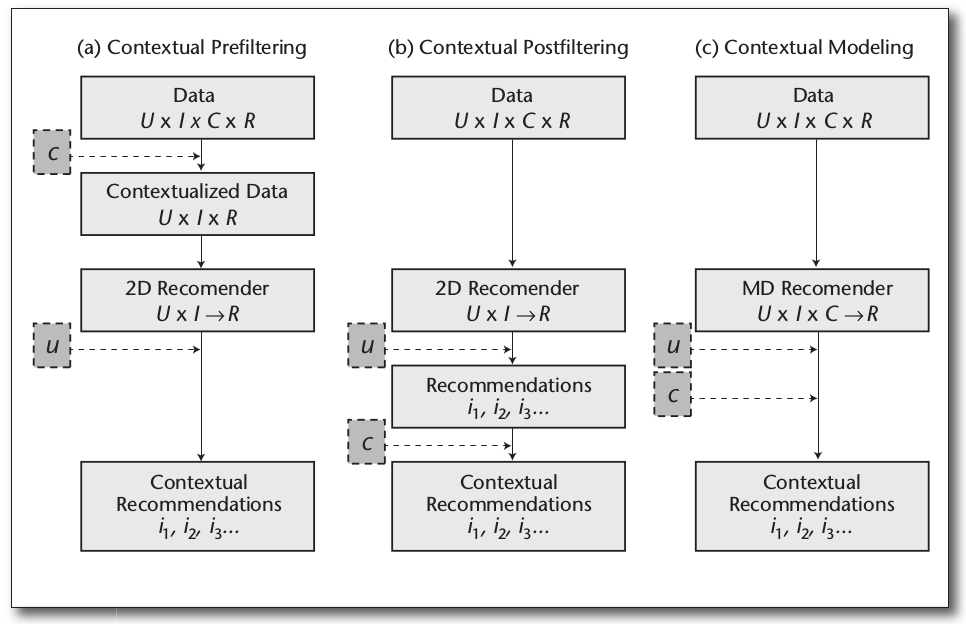
\includegraphics[width=\textwidth]{algo}
\end{figure*}


\subsubsection{Post-filtre contextuel}
~\\
Le post filtrage contextuel consiste à filtrer les résultats d'un algorithme
de recommandation classique à l'aide d'informations issues du
contexte\cite{DBLP:journals/tlt/VerbertMOWDBD12}. Il s'agit souvent d'adapter
ceux-ci de manière à incorporer des vecteurs de préférence utilisateur. Les
algorithmes de recommandation se déclinent en deux principales catégories, le
filtrage collaboratif et le filtrage sur contenu. \\

Le filtrage collaboratif désigne de façon générale les méthodes recommandant du
contenu à un utilisateur à partir d'informations issues du contexte du
comportement d'autres utilisateurs. Il s'agit de rechercher des clusters
d'utilisateurs aux comportements similaires susceptibles d'apprécier les mêmes
contenus, afin de pouvoir recommander à un membre du groupe ce que les autres
aiment déjà. La préférence d'un utilisateur pour un item peut être déterminée
de différentes manières. Elle l'est soit de manière explicite via une action 
d'évaluation de l'utilisateur. Dans le cas des systèmes de e-learning, cela
peut par exemple prendre la forme d'un formulaire de feedback ou d'un système
de vote. Elle aussi être déterminée indirectement, simplement par le fait qu'un
utilisateur consulte ou non une ressource. \\
\cite{Liou:2014:CPL:2617848.2617854} utilise par exemple les données issues du
système de  e-learning des internes d'un hôpital pour répartir les utilisateurs
en groupes afin de recommander de manière efficace des actions à effectuer sur
la plate-forme. Cette solution telle qu'elle est présentée comporte cependant
l'inconvénient de n'avoir été testée que sur des données d'archive et non en
temps réel. Peu d'informations sont précisées quant aux données utilisées dans
l'étude, notamment concernant leur taille.  \\

Les méthodes de filtrage basées sur le contenu reposent principalement sur
une modélisation des items à recommander ainsi que sur des profils utilisateurs
plus complets. \cite{DBLP:journals/jucs/SternKHKL10} présente par exemple une
méthode pour associer différents mots-clefs à des articles en vue de les
recommander à des utilisateurs avec lesquels les intérêts déterminés par
l'application correspondraient. \\

\subsubsection{Utilisation directe du contexte}
~\\
Certaines solutions se reposent directement sur des événements contextuels
pour proposer du contenu à celui-ci. Les types d'algorithmes utilisés varient
alors considérablement d'une solution à l'autre. La solution de formation en
entreprise APOSDLE utilise par exemple une représentation à base d'ontologie
pour représenter les tâches effectuées par un utilisateur lors de son travail
habituel ainsi que les compétences nécessaires pour les mener à
bien\cite{DBLP:journals/procedia/BehamKLL10}. Cette démarche consiste donc à
modéliser précisément les tâches qu'ont à effectuer les différents
collaborateurs d'une entreprise utilisateurs de la solution ainsi que les
compétences qu'elles mettent en jeu. Les relations entre tâches et compétences
sont également modélisées. L'application est capable d'évaluer le niveau de
compétence de chaque utilisateur par rapport à chacune de ces compétences à
partir des interactions de celui-ci avec les applications nécessaires à son
travail. L'outil peut alors recommander aux employés des collaborateurs experts
dans ces différentes compétences, à même de les aider dans leurs missions. \\

Une approche similaire est mise en place dans la solution d'apprentissage de
langues étrangères mobile PALLAS \cite{DBLP:conf/wmte/PetersenM06}. La position
de l'utilisateur est utilisée pour afficher des messages personnalisés en
fonction notamment de la langue étudiée et du niveau de l'utilisateur pour
inciter celui-ci à se rendre sur des points d'intérêt.
\cite{Kurti:2008:CMS:1456223.1456331} propose une approche similaire en ce que
le contexte utilisateur, notamment sa position, sert d'élément déclencheur à la
proposition d'activités d'apprentissage sur une solution mobile. \\

Des méthodes à base d'algorithmes génétiques sont également envisageables. En
modélisant les cours en ligne d'une université en tant que suite de sections
composées d'objets d'apprentissage de nature différentes,
\cite{smartECourseRecommander} recommande par exemple aux auteurs de ces cours
des nombres idéaux d'éléments comme des paragraphes, graphiques ou exercices à
y ajouter. En constatant l'importance des différents modes d'apprentissage dans
la capacité des étudiants à assimiler des connaissances, il y est assumé qu'une
variété d'items permette d'adapter les cours à ces différents types
d'apprentissage. Cette adéquation aux modes d'apprentissage est mesurée pour
chaque section de cours par des indicateurs basés sur la fréquence relative des
différents types d'objets les uns par rapport aux autres. Un algorithme
génétique est ensuite utilisé pour tester successivement différentes
compositions de cours afin d'optimiser leur faculté à être efficaces pour un
maximum de méthodes d'apprentissage. \\

\section{Application spécifique dans le domaine du e-learning}

\subsection{Les différents types de recommandation}

L'intérêt de la personnalisation des plate-formes de e-learning en fonction du
contexte utilisateur est de produire de façon générale des solutions de
meilleure qualité en rendant l'apprentissage plus efficace. Cette
personnalisation s'effectue notamment via des méthodes de recommandation qui se
différencient avant tout par la nature des objets recommandés. Des approches
très différentes ont en effet été imaginées, différents types de
recommandations pouvant être utilisés pour une même solution. \\

L'approche la plus courante retenue dans la personnalisation de systèmes
d'e-learning est la recommandation de ressources d'apprentissage
\cite{DBLP:journals/tlt/VerbertMOWDBD12}. Il peut s'agir d'items
complémentaires à la formation comme des exemples ou des éléments exercices
ayant pour but de faciliter l'apprentissage aux élèves, comme de cours complets
susceptibles de les intéresser. \\

L'on peut également envisager de recommander du contenu non pas à
l'étudiant, mais à l'auteur du cours \cite{smartECourseRecommander} dans
l'optique que celui-ci soit suffisamment pourvu en ressources variées lui
permettant de s'adapter le mieux possible aux différents modes d'apprentissages
des lecteurs. \\

Le postulat que l'aide apportée par des collègues est la meilleure stratégie
d'apprentissage sur le lieu de travail a par ailleurs motivé le développement
de solutions recommandant à l'utilisateur des collaborateurs experts dans des
domaines pour lesquels il manque de
connaissances\cite{DBLP:journals/procedia/BehamKLL10}.\\

Une autre approche parfois employée consiste à générer des messages
personnalisés encourageant l'utilisateur à se mettre en situation
d'apprentissage. Ce type de solution est notamment utilisé en conjonction sur
des plate-formes mobiles. \cite{DBLP:conf/wmte/PetersenM06}. \\

Dans le contexte d'une plate-forme de e-learning comportant des fonctionnalités
d'interaction entre différents utilisateurs, il devient envisageable de
suggérer à l'utilisateur d'effectuer de telles activités, comme poster un sujet
sur un forum intégré à la plate-forme après la consultation d'une ressource
\cite{Liou:2014:CPL:2617848.2617854}. \\

\subsection{Evaluation des différentes solutions}

Il est difficile de comparer les différents systèmes des recommandations
proposés par tous ces articles. Il y a plusieurs raisons à cela. Tout d'abord,
la plupart d'entre eux ne sont qu'à l'état de prototype et ont peu été testés
en situation réelle. D'autre part, les systèmes étudiés portent sur des
domaines très variés, et comme on l'a vu plus haut, ils ne recommandent pas
tous le même type de ressource. Certains systèmes recommandent des ressources
telles que de la documentation ou des exercices, alors que d'autres
recommandent des personnes, etc. Enfin, les méthodes et jeux de tests varient
grandement d'une étude à l'autre. \\

L'étude de Verbert et al. \cite{DBLP:journals/tlt/VerbertMOWDBD12} soulève ces
points et rapporte également quelques résultats de tests. Les évaluations ont
pu porter sur l'efficacité des systèmes à améliorer l'apprentissage, sur la
pertinence du contenu recommandé, ou encore sur l'utilité et des différents
systèmes. La plupart du temps, les systèmes semblent effectivement plus
efficaces que des méthodes plus traditionnelles, mais que cela peut dépendre du
domaine. La pertinence du contenu a pu être évaluée avec là encore diverses
méthodes, la plupart des systèmes évalués renvoyant de meilleurs résultats que
des systèmes de filtrage collaboratif classiques. Le sujet de l'utilité du
système a semble-t-il été mesuré pour plus de systèmes que les autres points,
et là encore avec des méthodes différentes. Si les différentes études
rapportent que les différents systèmes ont tous été perçus comme utiles,
beaucoup soulèvent également plusieurs problèmes d'ergonomie, et des
difficultés d'adaptation de la part des utilisateurs.\\

Le problème de l'absence de jeu de données standard est adressé par Draschsler
et al. \cite{DBLP:journals/procedia/DrachslerBVVDMBLSFW10}. Les auteurs
constatent qu'il n'existe aucun jeu de données pour tester les systèmes de
recommandation dans le contexte du e-learning -alors qu'il en existe pour les
systèmes commerciaux- et que le fait de créer des jeux de données standard
permettrait d'assurer la validité des expériences en favorisant la répétabilité
des tests. Ils soulignent la disparité des différents contextes
d'apprentissage, notamment d'une part les solutions s'adressant aux élèves
intégrés à un cursus formel comme une université par exemple, et d'autre part
les élèves apprenant en dehors du cadre d'un tel cursus.\\

Les auteurs proposent également plusieurs lignes de conduite à tenir lors du
choix des données : sélectionner des données représentatives des véritables
conditions d'utilisation, sélectionner des jeux de données concernant
suffisamment d'utilisateurs, et créer des jeux de données comparables les uns
aux autres, et donc partageant une structure similaire. Les auteurs
introduisent ensuite une approche générale pour créer les jeux de données,
étudient l'aspect juridique de la question quant à la protection de la vie
privée, et proposent un format standard d'échange des jeux de données.\\

\section{Conclusion}

Les plate-formes de e-learning couvrent des contextes d'apprentissage
différents, des cursus scolaires aux formations en entreprise, leur diversité
rend nécessaire l'adoption d'autant d'approches de personnalisations différentes,
nécessité exacerbée par un besoin d'accès mobile aux formations croissant.
Chaque utilisateur ayant des connaissances et des façons d'apprendre
différentes, il est d'autant plus pertinent d'adapter ces plate-formes pour
produire des applications plus efficaces prenant en compte des paramètres tels
que la position de l'utilisateur, sa formation ou ses habitudes
d'apprentissage.  La personnalisation de ces systèmes peut aussi bien se faire
en recommandant du contenu que des personnes de référence, tant aux professeurs
responsables de ces contenus qu'aux élèves. De nombreuses solutions ont été
développées pour adresser ces besoins, leur diversité rendant cependant la
tâche de comparer leurs résultats d'autant plus ardue. La personnalisation des
systèmes d'e-learning soulève un certain nombre de challenges, que ne facilitent
pas la difficulté de la mise en place de référentiels de données communs.

% references section

% can use a bibliography generated by BibTeX as a .bbl file
% BibTeX documentation can be easily obtained at:
% http://www.ctan.org/tex-archive/biblio/bibtex/contrib/doc/
% The IEEEtran BibTeX style support page is at:
% http://www.michaelshell.org/tex/ieeetran/bibtex/
\bibliographystyle{IEEEtran}
\bibliography{IEEEabrv,./ref.bib}

\end{document}
